

\section{String Basics}

\subsection{String Library}

\begin{frame}[fragile]
  \frametitle{String Basic Operations}
  {\smaller
    \begin{block}{String Representation}
      \begin{columns}[T]
        \column{0.45\textwidth}
\begin{verbatim}
// C/C++ (ends with '\0')
char[100] str;

#include<string>
str s;
\end{verbatim}
        \column{0.45\textwidth}
\begin{verbatim}
// JAVA
String str;

// JAVA strings are imutable!
// Modifying them = new object
\end{verbatim}
      \end{columns}
    \end{block}

    \begin{block}{Data Input}
      \begin{columns}[T]
        \column{0.45\textwidth}
\begin{verbatim}
// Word
scanf("%s",&str); cin >> str;

// Line
gets(str);
fgets(str,1000,strdin);
getline(cin,str);
\end{verbatim}
        \column{0.45\textwidth}
\begin{verbatim}
// Word
Scanner sc = new
       Scanner(System.in);
str = sc.next();

// Line
str = sc.nextLine();
\end{verbatim}
      \end{columns}
    \end{block}
  }
\end{frame}

% \begin{frame}[fragile]
%   \frametitle{String Basic Operations: A primer (2)}
%   {\smaller
%     \begin{block}{String Output and formatting}
%       \begin{columns}[T]
%         \column{0.45\textwidth}
% \begin{verbatim}
% // C/C++
% printf("s = %s, l = %d\n",
%    str, (int) strlen(str));
% cout << "s = " << str <<
%    ", l= " << str.length()
%    << endl;
% \end{verbatim}
%         \column{0.45\textwidth}
% \begin{verbatim}
% // JAVA
% System.out.print("..."); OR
% System.out.println(); OR
% System.out.printf(
%    "s = %s, l= %d\n", str,
%    str.length();)
% \end{verbatim}
%       \end{columns}
%     \end{block}
%     \begin{block}{Testing Two Strings for Equality}
%       \begin{columns}[T]
%         \column{0.45\textwidth}
% \begin{verbatim}
% result = strcmp(str,"test");
% result = (str == "test");
% \end{verbatim}
%         \column{0.45\textwidth}
% \begin{verbatim}
% result =
%    str.equals("test");
%
% \end{verbatim}
%       \end{columns}
%     \end{block}
%   }
% \end{frame}

\begin{frame}[fragile]
  \frametitle{String Basic Operations}
  {\smaller

      \begin{block}{Testing Two Strings for Equality}
\begin{verbatim}
// C/C++                         // JAVA
result = strcmp(str,"test");     result = str.equals("test");
result = (str == "test");
\end{verbatim}
      \end{block}


    \begin{block}{Combining Two or More Strings}
      \begin{columns}
        \column{0.45\textwidth}
\begin{verbatim}
strcpy(str,"hello");
strcat(str," world");
str = "hello";
str.append(" world");
\end{verbatim}
        \column{0.45\textwidth}
\begin{verbatim}
str = "hello";
str += " world";
// Careful!
// Creates new strings
\end{verbatim}
      \end{columns}
    \end{block}
    \begin{block}{Editing/Testing single characters in a string}
      \begin{columns}[T]
        \column{0.45\textwidth}
\begin{verbatim}
#include <ctype.h>
for (int i=0;str[i];i++)
   str[i] = toupper(str[i])
\end{verbatim}
        \column{0.45\textwidth}
\begin{verbatim}
// Java Strs are immutable
// create a new string
// or use StringBuffer
\end{verbatim}
      \end{columns}
    \end{block}
  }
\end{frame}

\begin{frame}[fragile]
  \frametitle{String Basic Operations}
  {\smaller
    \begin{block}{String Tokenizer -- Separates a string based on a character}
      \begin{columns}[T]
        \column{0.45\textwidth}
\begin{verbatim}
// C/C++
#include <string.h>
for (char *p.strtok(str," ");
     p; p=strtok(NULL," "))
   printf("%s",p)

#include <sstream>
stringstream p(str);
while (!p.eof()) {
  string token;
  p >> token;
  }
\end{verbatim}
        \column{0.45\textwidth}
\begin{verbatim}
// JAVA
import java.util.*;
StringTokenizer st = new
  StringTokenizer(str," ");
while (st.hasMoreTokens())
  System.out.println(
     st.nextToken());
\end{verbatim}
      \end{columns}
    \end{block}
    }
\end{frame}

\begin{frame}[fragile]
  \frametitle{String Basic Operations}
  {\smaller
    \begin{block}{Finding a Substring}
      \begin{columns}[T]
        \column{0.45\textwidth}
\begin{verbatim}
// C/C++
char *p=strstr(str,substr);
if (p) printf("%d",p-str-1);

int pos=str.find(substr);
if (pos!=string::npos)
  cout << pos-1 << endl;
\end{verbatim}
        \column{0.45\textwidth}
\begin{verbatim}
// JAVA
int pos =
  str.indexOf(substr);
if (pos != -1)
  System.out.println(pos);
\end{verbatim}
      \end{columns}
    \end{block}
    \begin{block}{Sorting Characters in a string}
      \begin{columns}[T]
        \column{0.45\textwidth}
\begin{verbatim}
#include <algorithm>
sort(s, s+(int)strlen(s));
sort(s.begin(),s.end());
\end{verbatim}
        \column{0.45\textwidth}
\begin{verbatim}
//Immutable, break the
//string using
//toCharArray()
\end{verbatim}
      \end{columns}
    \end{block}
  }
\end{frame}

% \begin{frame}[fragile]
%   \frametitle{String Basic Operations: A primer (6)}
%   {\smaller
%     \begin{block}{Sorting an array of strings or characters}
%       \begin{columns}[T]
%         \column{0.45\textwidth}
% \begin{verbatim}
% // C/C++
% #include <algorithm>
% #include <string>
% #include <vector>
% vector<string> s;
% // strings are put into s
% sort(s.begin(), s.end())
% \end{verbatim}
%         \column{0.45\textwidth}
% \begin{verbatim}
% // JAVA
% Vector<String> s =
%    new Vector<String>();
% Collections.sort(S);
%
% \end{verbatim}
%       \end{columns}
%     \end{block}
%   }
% \end{frame}

\subsection{Ad-Hoc String Problems}

\begin{frame}{Ad-hoc String Problems}
  Let's see some general string problems that can be solved using the string library functions that we just reviewed.\bigskip

  If you have difficulty in these problems, try using the {\bf Complete Search} approach on them first!
\end{frame}

\begin{frame}
  \frametitle{Immediate Decodability}
    \begin{exampleblock}{Problem Outline}
      Given a set of {\bf 2 to 8 binary words}, of length
      between {\bf 1 and 10}, decide if the set is {\bf immediately
      decodable}. \bigskip

      Immediate decodable means {\bf no word is a prefix of
      another word}.
    \end{exampleblock}

    \begin{columns}
      \column{0.5\textwidth}
      {\bf Input example 1 (Decodable)}
      \begin{itemize}
        \item 001
        \item 110
        \item 10101
        \item 01101
        \item 100
      \end{itemize}
      \column{0.5\textwidth}
      {\bf Input example 2 (not decodable)}
      \begin{itemize}
        \item {\bf 001}
        \item 10101
        \item {\bf 00101}
        \item 11011
        \item 1011
      \end{itemize}
    \end{columns}\medskip

    {\bf QUIZ:} How do you solve this problem?
\end{frame}



\begin{frame}{Immediate Decodability}{Hints}
  \begin{columns}
    \column{0.5\textwidth}
    {\bf Input example 1 (Decodable)}
    \begin{itemize}
      \item 001
      \item 110
      \item 10101
      \item 01101
      \item 100
    \end{itemize}
    \column{0.5\textwidth}
    {\bf Input example 2 (not decodable)}
    \begin{itemize}
      \item {\bf 001}
      \item 10101
      \item {\bf 00101}
      \item 11011
      \item 1011
    \end{itemize}
  \end{columns}\bigskip

  \begin{itemize}
    \item A simple way to solve is to test every pair of strings, to see if one is a prefix of another;
    \begin{itemize}
      \item What is the difference between prefix and substring?
      \item How many steps this algorithm takes?
    \end{itemize}
    \item You can improve this algorithm if you reduce the number of comparisons;
    \begin{itemize}
      \item How can you prune the algorithm?
      \item Does the order of the strings matter?
    \end{itemize}
  \end{itemize}
\end{frame}


\begin{frame}[fragile]
  \frametitle{Ad-hoc Problem 2 -- Caesar Cypher}
    \begin{exampleblock}{Problem Outline}
      {\small A {\bf rotational cypher} transforms \emph{plaintext} to
      \emph{cyphertext} by adding a constant value "k" to every character.\medskip

      Example: I LOVE YOU + ($k = 3$) $\rightarrow$ LCORYHCARY\medskip

      Given a dictionary of plaintext, find the best translation of
      the cyphertext.}
    \end{exampleblock}

\begin{verbatim}
THIS  DAWN  THAT   || INPUT:  BUUBDLA PSSPABUAEBXO
ZORRO OTHER AT     || OUTPUT: ATTACK ZORRO AT DAWN
THING THE
\end{verbatim}
{\bf QUIZ}: How do we solve this problem?
\end{frame}

\begin{frame}[fragile]{Ad-hoc Problem 2 -- Caesar Cypher}
\begin{verbatim}
  THIS  DAWN  THAT   || INPUT:  BUUBDLA PSSPABUAEBXO
  ZORRO OTHER AT     || OUTPUT: ATTACK ZORRO AT DAWN
  THING THE
\end{verbatim}

  \begin{itemize}
    \item Our objective is to find the rotation that fits the largest number of words in the dictionary.\bigskip

    \item Try every rotation, for each rotation see if the words are substrings.\bigskip

    \item This is a very slow approach. Can it be faster?
  \end{itemize}
\end{frame}

% \begin{frame}[fragile]
%   \frametitle{Discussion of Ad-hoc problems}
%
%     \begin{exampleblock}{Problem 3 -- Ensuring Truth}
%       Given a boolean formula in the following format, is the formula
%       {\bf satisfiable}?
%
%       \begin{equation*}
%         (x_1\land \hat{x_2}\land \ldots \land {x_n}) \lor (x_i\land \hat{x_j}\land\ldots) \lor \ldots
%       \end{equation*}
%
%       {\bf Examples:}
% \begin{verbatim}
% (a&b&c)|(a&b)|(a)        <--- Satisfiable;
% (x&~x)                   <--- Not satisfiable;
% \end{verbatim}
%     \end{exampleblock}
%
%     \begin{itemize}
%       \item A big part of the program is to build a function to read a string with size over 5000 in the right format.
%       \item SAT is a very hard problem, but for this particular string format, is there a simple way to calculate satisfiability?
%     \end{itemize}
% \end{frame}


\section{String Matching} % (6.4)
\subsection{Basics}

\begin{frame}[fragile]{String Matching}
  \begin{block}{Definition}
    Given a string $T$ (also called {\bf text}), we want to test if the substring $P$ (also called {\bf pattern}) exists in $T$.
    \bigskip

    If $P$ exists in $T$, we want to know the {\bf index} of the start of $P$ in $T$.
  \end{block}\bigskip

  Example:
\begin{verbatim}
T: STEVEN EVENT
P: EVE            indexes: 2 and 7
P: EVENT          indexes: 7
P: EVENING        indexes: -1 or NULL
\end{verbatim}
\end{frame}

\begin{frame}{String Matching and Libraries}

  \begin{block}{How do we solve string matching problems?}
    {\bf Use your language's string library!}
    \begin{itemize}
      \item In C/C++: strstr(T,P) or T.find(P)
      \item In Java: T.indexOf(P)
    \end{itemize}\bigskip

    No bugs! Usually very efficient!
  \end{block}\bigskip

  But...
  \begin{itemize}
    \item Maybe you have a specific matching function (1 equals I)
    \item Maybe your string changes over time;
    \item Maybe you have to match multiple strings at the same time;
    \item Maybe you have to string match in a graph;
    \item etc...
  \end{itemize}\bigskip

  So it is useful to know how to implement string matching
\end{frame}

\begin{frame}[fragile]{String Matching: Complete Search}

  For every character $T_i$, test if $P$ begins at that position.\bigskip

\begin{verbatim}
for (int i = 0; i < |T|; i++)
  bool match = true;
  for (int j = 0; j < |P| && match; j++)
    if (i+j >= |T| || P[j] != T[i+j])
      match = false;
  if (match)
    printf("Match P at index %d\n", i);
\end{verbatim}

{\bf Number of Steps}:
  \begin{itemize}
    \item Average case: $O(n)$ -- For natural T and small P;
    \item Worst case: $O(mn)$ -- For programming challenges;
    \begin{itemize}
      \item T = AAAAAAAAAAAAB
      \item P = AAAAAAAB
    \end{itemize}
  \end{itemize}
\end{frame}

\subsection{Knuth-Morris-Pratt}
\begin{frame}[fragile]
  \frametitle{The Knuth-Morris-Pratt (KMP) Algorithm}

  \begin{itemize}
    \item The naive algorithm can be very expensive if the prefix of $P$ happens many times in $T$.
    \item In 1977, Knuth, Morris and Pratt developed an algorithm that {\bf uses these prefixes} to realize fast string matching.
  \end{itemize}

  \begin{block}{Basic Idea}
    \begin{itemize}
    \item The KMP algorithm works by identifying "borders" in the partial match between $P$ and $T$.
    \item These borders are characterized by identical prefixes and sufixes in the T-P match.
    \item The algorithm uses these matches to advance the indexes of $T$ and $P$, greatly reducing the number of comparisons.
  \end{itemize}
  \end{block}
  The KMP algorithm is O(P+T).
\end{frame}

\begin{frame}[fragile]{KMP Algorithm -- Simulation}

{\smaller
\begin{verbatim}
              1         2         3         4         5
    012345678901234567890123456789012345678901234567890
T = I DO NOT LIKE SEVENTY SEV BUT SEVENTY SEVENTY SEVEN
P = SEVENTY SEVEN
// for i from 0 to 13, KMP works like full search

                  SEVENTY SEVEN
// Here, the collision is at i=25, j = 11, But because "SEV" is
// a "border", i stays the same and j is rewinded to 3

                                  SEVENTY SEVEN
// Here we find a match with i=43, j=13; SEVEN is a border, so j
// is rewinded to 5, and i is kept the same. The algorithm
// continues matching at i=44, j=5 ("T")

                                          SEVENTY SEVEN
// KMP finds a second match
\end{verbatim}}

\end{frame}


\begin{frame}[fragile]{KMP Algorithm -- Rewind Array}

\begin{block}{}
To avoid repeated matches, the KMP algorithm builds a {\bf rewind table} $b$ (back).

\begin{verbatim}
     0 1 2 3 4 5 6 7 8 9 0 1 2 3
P =  S E V E N T Y   S E V E N \0
b = -1 0 0 0 0 0 0 0 0 1 2 3 4 5
\end{verbatim}

Following the table $b$, we know that if we find a mismatch at $j = 11$, then we need to rewing $j$ to $b[11] = 3$ to continue matching.\bigskip

The text index $i$, on the other hand, will stay the same, and go forward by 1 if $b[j] = -1$.
    \end{block}
\end{frame}

\begin{frame}[fragile]{KMP Algorithm -- PseudoCode}

  {\smaller
  \begin{exampleblock}{}
\begin{verbatim}
char T[MAX_N], P[MAX_N];
int b[MAX_N], n, m;

void kmpPreprocess() {     // Create the Back Array
  int i = 0, j = -1; b[0] = -1;
  while (i < m) {
     while (j >= 0 && P[i] != P[j]) j = b[j];
     i++; j++;
     b[i] = j; }}

void kmpSearch() {         // Search the substring
  int i = 0, j = 0;
  while (i < n) {
     while (j >= 0 && T[i] != P[j]) j = b[j];
     i++; j++;
     if (j == m) {
        printf("P is found at index %d in T\n", i - j);
        j = b[j]; }}}
\end{verbatim}
  \end{exampleblock}
  }
\end{frame}

\subsection{Z algorithm}

\begin{frame}[fragile]{String Matching with the Z-Algorithm}
  Another linear algorithm that can perform string matching is the {\bf Z algorithm}.\bigskip

  The Z algorithm constructs a {\bf Z array}. For every index $i\in S$, $Z[i]$ is the size of the prefix of $S$ that begins in $i$.\bigskip

\begin{verbatim}
T = AASABAABAAT, P = AAB, S = P$T

... Build Z Array ...
S   = AAB$AASABAABAAT
Z[S]= X10021010310210
               ^
               String matched here. Z[i] = Len(P)
\end{verbatim}
\end{frame}

\begin{frame}[fragile]{Z-Algorithm -- Pseudocode}
  \begin{block}{}
{\smaller
\begin{verbatim}
void Zarray(string S, int Z[]) {
    int n = S.length(); int L, R, k;
    L = R = 0;             // Prefix counters
    for (int i = 1; i < n; i++) {
        if (i > R) {       // Full search of prefix
            L = R = i;
            while (R < n && S[R] == S[R-L]) R++;
            Z[i] = R-L; R--;
        } else {           // Inside prefix candidate
            k = i-L;
            if (Z[k] < R-i+1) Z[i] = Z[k]; // no extension
            else {                         // prefix extension
                L = i;
                while (R < n && S[R] == S[R-L]) R++;
                Z[i] = R-L; R--;
}   }   }   }
\end{verbatim}}
  \end{block}

{\smaller {\bf Simulation:}
\url{https://personal.utdallas.edu/~besp/demo/John2010/z-algorithm.htm}}

\end{frame}

\begin{frame}{Z algorithm or KMP algorithm?}
  Should you use the Z algorithm or the KMP algorithm?\bigskip

  \begin{itemize}
    \item Both algorithms have the same time complexity: $O(T+P)$\bigskip

    \item Which algorithm is easier to understand?
    \begin{itemize}
      \item KMP calculates a recursive suffix state machine for P;
      \item Z-algorithm calculates a substring size array for T;
    \end{itemize}\bigskip
  \end{itemize}
\end{frame}



\section{String Algorithms with DP} % (6.5)
\begin{frame}{String Algorithms with Dynamic Programming}
  \begin{block}{}
    Some string problems can be described as a {\bf search problem}. In this section, we will introduce two common problems in programming challenges that can be solved with DP algorithms:\bigskip

    \begin{itemize}
    \item String Alignment/Edit Distance
    \item Longest Common Subsequence
    \end{itemize}
  \end{block}
  \bigskip

  It is interesting to note that substring matching is also a search problem, and that KMP / Z-algorithms can be seen as a kind of memoization.
\end{frame}

\subsection{String Alignment}
\begin{frame}[fragile]{String DP: String Alignment}

The {\bf String Alignment}\footnote{Also called Edit Distance or Levenhstein Distance, used by spellchecking algorithms!} problem is defined as follows. Align two strings, A and B, with the maximum "alignment score":\bigskip

\begin{itemize}
  \item Character A[i] and B[i] match: do nothing, score +2
  \item Character A[i] and B[i] mismatch: replace A[i], score -1
  \item Insert a space in A[i]: score -1
  \item Delete A[i] (equals to insert in B[i]): score -1
\end{itemize}

\begin{verbatim}
               non-optimal    optimal
A: ACAATCC   | A_CAATCC     | A_CAATCC
B: AGCATGC   | AGCATGC_     | AGCA_TGC
score:       | 2-22--2- = 4 | 2-22-2-2 = 7
\end{verbatim}\bigskip

\end{frame}


\begin{frame}[fragile]{String Alignment: Bottom Up DP}
  \begin{verbatim}
                 non-optimal    optimal
  A: ACAATCC   | A_CAATCC     | A_CAATCC
  B: AGCATGC   | AGCATGC_     | AGCA_TGC
  score:       | 2-22--2- = 4 | 2-22-2-2 = 7
  \end{verbatim}
  The {\bf Full search} approach requires recursively testing each of three options for each A[i] ($O(3^n)$). We can solve this in $O(n^2)$ using DP:

  \begin{itemize}
    \item $V(i,j)$: optimal score for prefix $A[1..i],B[1..j]$
    \item Start condition:
    \begin{itemize}
      \item $V(0,0) = 0$ \hspace{1cm} (Do nothing)
      \item $V(i,0) = -1\times i$, $V(0,j) = -1\times j$ \hspace{1cm} (delete A or B)
    \end{itemize}
    \item Recurrence: $V(i,j) = \text{max}(C_1, C_2, C_3)$, where
    \begin{itemize}
      \item $C_1 = V(i-1, j-1) + \text{score}(A[i],B[j])$ // Score of match/mismatch;
      \item $C_2 = V(i-1,j) + \text{score}(A[i],\_)$ \hspace{1cm}// Delete $A[i]$;
      \item $C_3 = V(i,j-1) + \text{score}(\_,B[j])$ \hspace{1cm}// Delete $B[j]$;
    \end{itemize}
  \end{itemize}
\end{frame}


\begin{frame}[fragile]{String Alignment: Bottom Up DP}{Simulation Matching AGCATGC and ACAATCC}

\begin{itemize}
  \item Recurrence: $V(i,j) = \text{max}(C_1, C_2, C_3)$, where
  \begin{itemize}
    \item $C_1 = V(i-1, j-1) + \text{score}(A[i],B[j])$ // Score of match/mismatch;
    \item $C_2 = V(i-1,j) + \text{score}(A[i],\_)$ \hspace{1cm}// Delete $A[i]$;
    \item $C_3 = V(i,j-1) + \text{score}(\_,B[j])$ \hspace{1cm}// Delete $B[j]$;
  \end{itemize}
\end{itemize}

\begin{verbatim}
   |  _ |  A |  G |  C |  A |  T |  G |  C |
 _ |  0 | -1 | -2 | -3 | -4 | -5 | -6 | -7 |
 A | -1 |
 C | -2 |
 A | -3 |
 A | -4 |
 T | -5 |
 C | -6 |
 C | -7 |
\end{verbatim}

\end{frame}


\subsection{Longest Common Subsequence in String}

\begin{frame}[fragile]
  \frametitle{Longest Common Subsequence in Strings}
    \begin{block}{Problem Definition}
      Given strings $A$ and $B$, what is their longest common subsequence?\medskip

\begin{verbatim}
A  :   'ACAATCC'     - A_CAAT_CC
B  :   'AGCATGC'     - AGCA_TGC_
LCS:    AC AT C      - A_CA_T_C_ : ACATC
\end{verbatim}
    \end{block}\bigskip

  \begin{itemize}
    \item We can solve LCS using a modification of String Aligment;
    \item Use String Alignment DP, but change costs:
    \begin{itemize}
      \item Cost of Mismatch: $-\infty$
      \item Cost of insert/deletion: $0$
      \item Cost of Matching: $1$
    \end{itemize}
  \end{itemize}
\end{frame}

\begin{frame}
  \frametitle{Longest Palindrome}
    \begin{block}{Problem Description}
      A {\bf palindrome} is a string $S$ where $S = \text{rev}(S)$. For example: MADAM.\bigskip

      Given a string $T$, what is the {\bf longest palindrome} that you can create by deleting characters from $T$?
    \end{block}

    Examples:
    \begin{itemize}
    \item ADA\alert{M} -- ADA
    \item MADAM -- MADAM
    \item NEVERODDOREVEN\alert{ING} -- NEVERODDOREVEN
    \item RACE\alert{F1}CAR\alert{FAST} -- RACECAR
    \end{itemize}\bigskip

    {\bf QUIZ:} Can you solve with Full Search? String Alignment DP? Others?
  \end{frame}

\begin{frame}
  \frametitle{Longest Palindrome}
    \begin{block}{Problem Description}
      Given a string $S$ of size up to $N = 1000$ characters, what is the
      longest palindrome that you can make by deleting characters from $S$?
    \end{block}

    DP Solution:
    \begin{itemize}
    \item State Table:
      {\smaller
      \begin{itemize}
      \item len(i,j) - The largest palindrome found between $i$ and $j$
      \end{itemize}}
    \item Start Conditions:
      {\smaller
      \begin{itemize}
        \item If $l=r$ then len$(l,r)=1$.
        \item If $r=l+1 \text{ and } S[l]=S[r]$, len$(l,r)=2$, else len$(l,r)=1$.
      \end{itemize}}
    \item Transition:
      {\smaller
      \begin{itemize}
        \item If $S[l]=S[r]$, then len$(l,r)=2+\text{len}(l+1,r-1)$;
        \item else $\text{len}(l,r) = \text{max}(\text{len}(l+1,r),\text{len}(l,r-1))$
      \end{itemize}}
    \end{itemize}

    This DP has complexity $O(n^2)$
\end{frame}

\begin{frame}[fragile]
  \frametitle{Longest Palindrome}

  Longest Palindrome DP: Diagonal Table Top Down

  {\smaller
\begin{verbatim}

       len(l,r)               len(l,r)         transition:
      final state           initial state   - A[l] == A[r]?
                                              len(l+1,r-1)+2
  R A C E F 1 C A R     R A C E F 1 C A R   - A[1] != A[r]?
                                              max(left,down)
R 1 1 1 1 1 1 3 5 7   R 1 1
A   1 1 1 1 1 3 5 5   A   1 1
C     1 1 1 1 3 3 3   C     1 1
E       1 1 1 1 1 1   E       1 1
F         1 1 1 1 1   F         1 1
1           1 1 1 1   1           1 1
C             1 1 1   C             1 1
A               1 1   A               1 1
R                 1   R                 1

\end{verbatim}

  }
\end{frame}


\section{Suffix Trie/Array} % (6.6)
\subsection{Outline}
\begin{frame}
  \frametitle{Suffix Trie: Definition}

  {\smaller
    \begin{block}{Definition}
      Data structure used to find matching suffixes of multiple strings.
    \end{block}

    \vfill

    \begin{center}
    \structure{Suffix Trie for \{'CAR','CAT','RAT'\}}
    \end{center}

    \vfill

    \begin{columns}[T]
      \column{0.25\textwidth}
      All Suffixes
      \begin{enumerate}
      \item CAR
      \item AR
      \item R
      \item CAT
      \item T
      \item RAT
      \item AT
      \item T
      \end{enumerate}
      \column{0.25\textwidth}
      Sorted, Unique Suffixes
      \begin{enumerate}
      \item AR
      \item AT
      \item CAR
      \item CAT
      \item R
      \item RAT
      \item T
      \end{enumerate}
      \column{0.45\textwidth}
      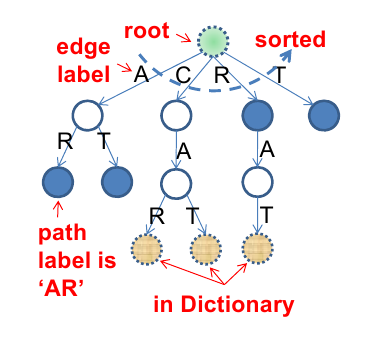
\includegraphics[width=.9\textwidth]{../img/suffixtrie_halim}\\
      % TODO: Replace suffix trie image with one of my own design
    \end{columns}
  }
\end{frame}

\begin{frame}
  \frametitle{Suffix Trie: Using it for a single, long string}
  {\smaller
  \begin{center}
    \structure{Suffix Trie (T='GATAGACA\alert{\$}')}
  \end{center}
  \begin{columns}[T]
    \column{0.35\textwidth}

    Create all $n$ suffixes:

    \begin{tabular}{c|l}
      i & suffix\\
      \hline
      0 & GATAGACA\$\\
      1 & ATAGACA\$\\
      2 & TAGACA\$\\
      3 & AGACA\$\\
      4 & GACA\$\\
      5 & ACA\$\\
      6 & CA\$\\
      7 & A\$\\
      8 & \$\\
    \end{tabular}

    Count the occurence of substring $m$:
    \begin{itemize}
    \item 'A': 4 times
    \item 'GA': 2 times
    \item 'AA': 0 times
    \end{itemize}
    \column{0.65\textwidth}
    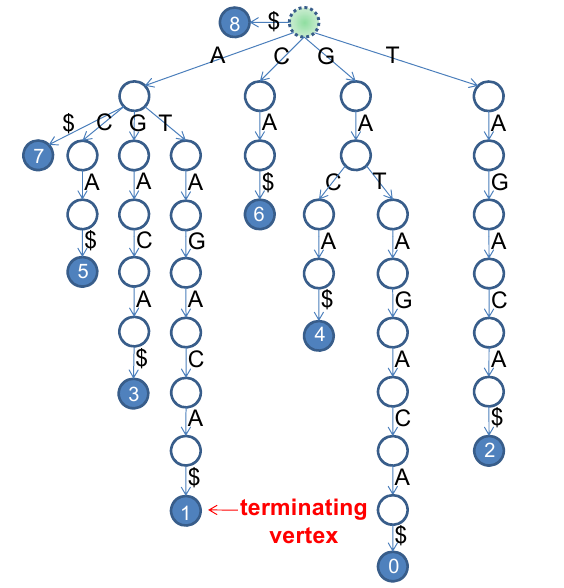
\includegraphics[width=.9\textwidth]{../img/suffixtrie_halim2}
  \end{columns}
  }
\end{frame}

\begin{frame}
  \frametitle{Suffix Trie: Suffix Tree}
  {\smaller
  \begin{center}
    \structure{Suffix Trie (T='GATAGACA\alert{\$}')}\\
    Compress single child nodes to obtain ``Suffix Tree''
  \end{center}
  \begin{columns}[T]
    \column{0.35\textwidth}

    \begin{tabular}{c|l}
      i & suffix\\
      \hline
      0 & GATAGACA\$\\
      1 & ATAGACA\$\\
      2 & TAGACA\$\\
      3 & AGACA\$\\
      4 & GACA\$\\
      5 & ACA\$\\
      6 & CA\$\\
      7 & A\$\\
      8 & \$\\
    \end{tabular}

    \bigskip

    With the suffix tree, many algorithms become faster.


    \column{0.65\textwidth}
    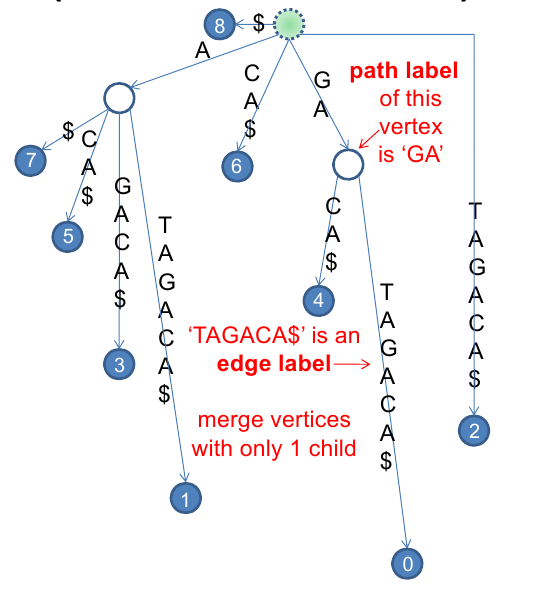
\includegraphics[width=.9\textwidth]{../img/suffixtree_halim}
    \ppagenote{Suffix Tree/Array images from Steven Halim, "Competitive Programming 3", chapter 6.6}
  \end{columns}
  }
\end{frame}

\subsection{Uses of a Suffix Tree}
\begin{frame}
  \frametitle{Uses of a Suffix Tree 1: String Matching} {\smaller

    \structure{Assuming that we have the Suffix Tree already built},
    we can find all occurrences of substring $m$ in $T$ in time
    $O(m+\text{occ})$, where occ is the number of occurrences.

  \begin{center}
    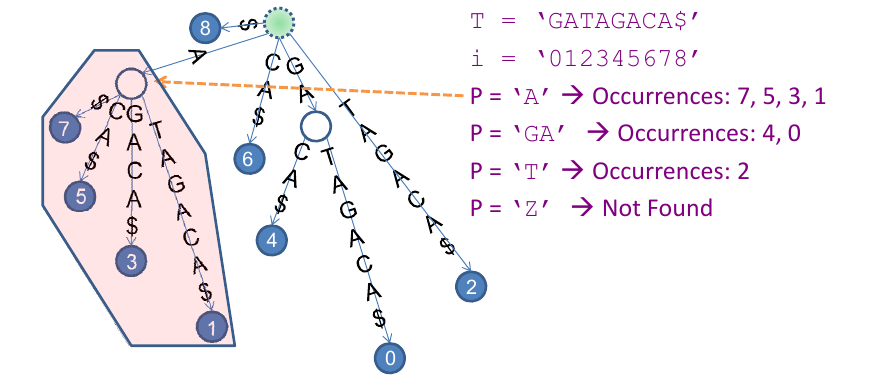
\includegraphics[width=0.9\textwidth]{../img/stringmatching_halim}
  \end{center}
  }
\end{frame}

\begin{frame}
  \frametitle{Uses of a Suffix Tree 2: Longest Repeated Substring}
  {\smaller
  \begin{itemize}
  \item The LRS is the longest substring with number of occurrences $> 2$;
  \item The LRS is the deepest internal node in the tree;
  \end{itemize}

  \begin{center}
    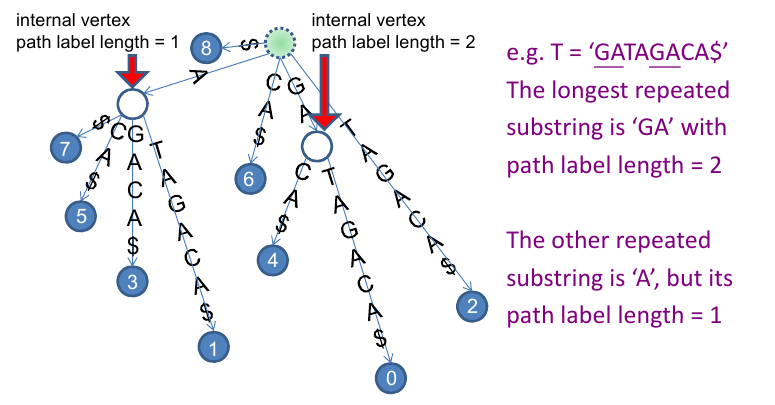
\includegraphics[width=0.9\textwidth]{../img/longestrepeatingsubstring_halim}
  \end{center}
  }
\end{frame}

\begin{frame}
  \frametitle{Uses of a Suffix Tree 3: Longest Common Substring}
  {\smaller
    \begin{itemize}
    \item We can find the common substring of $M$ and $N$ by making a
      combined Suffix Tree. Each string has a different ending
      character.
    \item The common substring is the deepest node that has both characters.
    \end{itemize}
  \begin{center}
    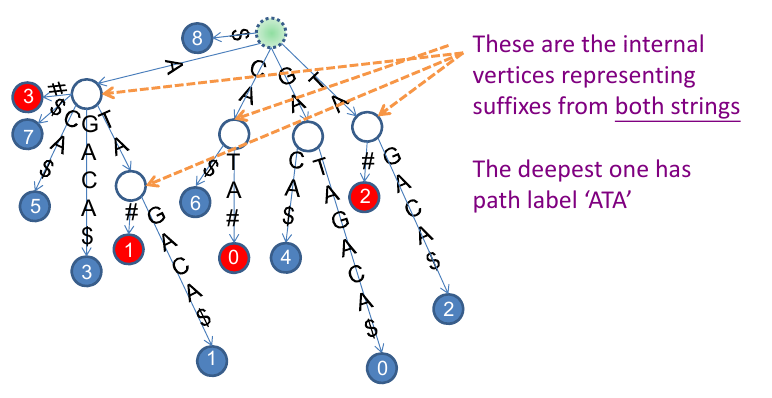
\includegraphics[width=0.9\textwidth]{../img/longestcommonsubstring_halim}
  \end{center}
  }
\end{frame}

\subsection{Suffix Array}
\begin{frame}
  \frametitle{Suffix Trie: Suffix Array (1)}
  {\small
  \begin{itemize}
    \item The algorithms in previous slides are very efficient...\\
      ... \structure{if you have the suffix tree}

      \medskip

    \item The suffix tree can be built in $O(n)$...\\
      ... but implementation is rather complex;

      \medskip

    \item In this course, we will see the \structure{Suffix Array};

      \medskip

    \item The Suffix Array is built in $O(n\log{n})$...\\
      ... but the implementation is very simple!
  \end{itemize}

  \vfill

  \begin{block}{}
    I encourage you to study the implementation of the suffix tree by yourself!
  \end{block}
  }
\end{frame}

\begin{frame}
  \frametitle{Suffix Trie: Suffix Array (2)}

  {\smaller

    \begin{itemize}
    \item To make a Suffix array, make an array of all possible
      suffixes of $T$, and sort it;
    \item The order of the suffix array is the
      \structure{visit in preorder} of the suffix tree;
      % TODO: Japanese for pre-order visit
    \item We can adapt all algorithms accordingly;
    \end{itemize}

  \begin{columns}
    \column{0.4\textwidth}
    \begin{tabular}{c|l}
      i & suffix\\
      \hline
      0 & GATAGACA\$\\
      1 & ATAGACA\$\\
      2 & TAGACA\$\\
      3 & AGACA\$\\
      4 & GACA\$\\
      5 & ACA\$\\
      6 & CA\$\\
      7 & A\$\\
      8 & \$\\
    \end{tabular}
    \column{0.2\textwidth}
    Sort $\rightarrow$
    \column{0.4\textwidth}
    \begin{tabular}{c|c|l}
      i & SA[i] & suffix \\
      \hline
      0 & 8 & \$\\
      1 & 7 & A\$\\
      2 & 5 & ACA\$\\
      3 & 3 & AGACA\$\\
      4 & 1 & ATAGACA\$\\
      5 & 6 & CA\$\\
      6 & 4 & GACA\$\\
      7 & 0 & GATAGACA\$\\
      8 & 2 & TAGACA\$\\
    \end{tabular}
  \end{columns}
  }
\end{frame}

\begin{frame}[fragile]
  \frametitle{Suffix Array: Implementation (1)}
  {\smaller
    \begin{exampleblock}{Simple Implementation}
\begin{verbatim}
#include <algorithm>
#include <cstdio>
#include <cstring>
using namespace std;
char T[MAX_N]; int SA[MAX_N],i,n;

bool cmp(int a, int b) { return strcmp(T+a, T+b) < 0; }
// O(n)

int main() {
  n = (int) strlen (gets(T));
  for (int i = 0; i < n; i++) SA[i] = i;
  sort (SA, SA+n, cmp); // O(n^2 log n) }
\end{verbatim}
    \end{exampleblock}

    This implementation is too slow for strings bigger than 1000 characters.
  }
\end{frame}

\begin{frame}[fragile]
  \frametitle{Suffix Array: Implementation (2.1)}
  {\smaller
    \begin{exampleblock}{O(n log n) implementation using ``ranking pairs/radix sort''}
\begin{verbatim}
char T[MAX_N]; int n; int c[MAX_N];
int RA[MAX_N], tempRA[MAX_N], SA[MAX_N], tempSA[MAX_N];

void countingSort(int k) {
  int i, sum, maxi = max(300,n); //255 ASCII chars or n
  memset(c, 0, sizeof(c));
  for (i = 0; i < n; i++) c[i+k<n? RA[i+k] : 0]++
  for (i = sum = 0; i < maxi; i++)
    { int t = c[i]; c[i] = sum; sum += t;} //frequency
  for (i = 0; i < n; i++)
    tempSA[c[SA[i]+k < n ? RA[SA[i]+k] : 0]++] = SA[i];
  for (i = 0; i < n; i++) // update suffix array
    SA[i] = tempSA[i];
}

// ... continues next slide
\end{verbatim}
    \end{exampleblock}
  }
\end{frame}

\begin{frame}[fragile]
  \frametitle{Suffix Array: Implementation (2.2)}
  {\smaller
    \begin{exampleblock}{O(n log n) implementation using ``ranking pairs/radix sort''}
\begin{verbatim}
// ... continued from last slide

void constructSA() {
  int i, k, r;
  for (i = 0; i < n; i++) { RA[i] = T[i]; SA[i] = i;}
  for (k = 1; k < n; k <<=1) {
    countingSort(k); countingSort(0);
    tempRA[SA[0]] = r = 0;
    for (i = 1; i < n; i++) tempRA[SA[i]] =
           (RA[SA[i]] == RA[SA[i-1]] &&
            RA[SA[i]+k] == RA[SA[i-1]+k]) ? r : ++r;
    for (i = 0; i < n; i++)
      RA[i] = tempRA[i];
    if (RA[SA[n-1]] == n-1) break;
}}
\end{verbatim}
    \end{exampleblock}
  }
\end{frame}

\begin{frame}
  \frametitle{Suffix Array: Using Suffix Array (1)}
  {\smaller
    \begin{block}{String Matching: Finding 'GA'}
      \begin{itemize}
      \item Do a binary search once to find the lower bound;
      \item Do a binary search once to fint the upper bound;
      \end{itemize}
    \end{block}
    \begin{center}
      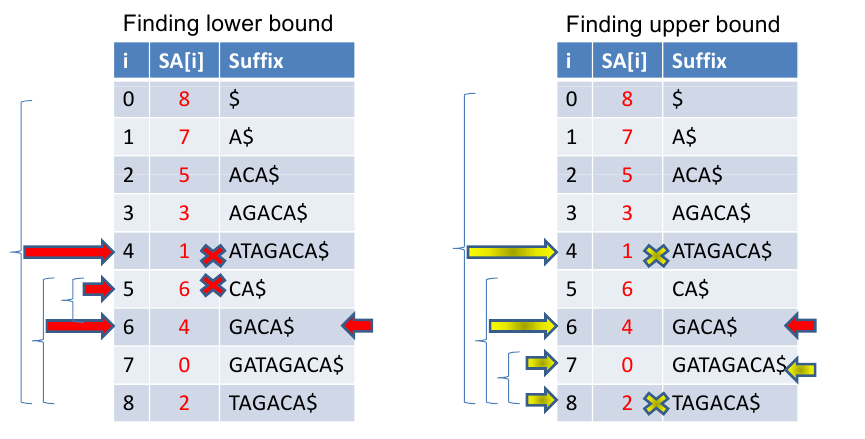
\includegraphics[width=0.9\textwidth]{../img/suffixarray_halim}
    \end{center}
  }
\end{frame}

\begin{frame}
    \frametitle{Suffix Array: Using Suffix Array (2)}
  {\smaller
    \begin{block}{Longest Repeated Substring}
      Find the longest common prefix between suffix $i$ and $i+1$
    \end{block}
    \begin{center}
      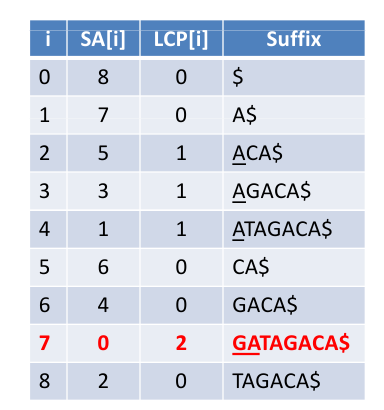
\includegraphics[width=0.5\textwidth]{../img/suffixarray2_halim}
    \end{center}
  }
\end{frame}

\begin{frame}
    \frametitle{Suffix Array: Using Suffix Array (3)}
  {\smaller
    \begin{block}{Longest Common Substring}
      \begin{itemize}
      \item Create Suffix Array for appended strings $MN$;
      \item Find the longest common prefix that has both string enders;
      \end{itemize}
    \end{block}
    \begin{center}
      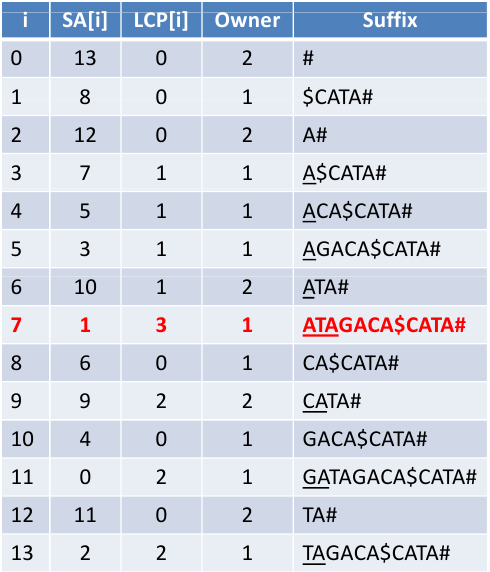
\includegraphics[width=0.45\textwidth]{../img/suffixarray3_halim}
    \end{center}
  }
\end{frame}
